\documentclass[../user-manual.tex]{subfiles}

\begin{document}
	В данной главе рассматриваются вопросы работы со встроенными в систему Магрепорт сводными таблицами. Все примеры построены на основе объектов, создаваемых в качестве учебных примеров в главе \ref{chapter:developing}.
	
	На основе данных плоской таблицы выполненного отчета вы можете создать сводную таблицу и производить анализ данных при помощи её инструментария. Сводная таблица позволяет вычислять агрегированные значения, соответствующие значениям измерений, расположенных в строках и столбцах таблицы.
	
	\begin{concept}
		Сводные таблицы являются мощнейшим инструментом оперативного анализа данных, позволяя в режиме интерактивного взаимодействия с платформой проводить операции агрегации и фильтрации. Поэтому мы в Магрепорт уделяем много внимания развитию функционала сводных таблиц. Сводные таблицы встречаются в различных инструментах анализа данных, в частности этот инструмент представлен в Excel и является одной из наиболее востребованных его функций. Мы придерживаемся устоявшейся терминологии, в которой поля данных, расположенные по строкам и столбцам сводной таблицы, по которым осуществляется агрегация, называются \textit{измерениями}, а агрегированные значения полей, которые вычисляются в разрезе данных измерений --- \textit{метриками}.
	\end{concept}
	
	Для перехода в область работы со сводными таблицами, в меню выполненного отчета необходимо нажать на кнопку <<Сводная таблица>> (см. рис. \ref{fig:open-pivot-button}).
	
	\begin{figure}[h]
		\centering
		
\includegraphics[width=\graphicswidth]{img/1-open-pivot-button.png}
		\caption{Кнопка перехода в сводную таблицу}
		\label{fig:open-pivot-button}
	\end{figure}	
	
	\section{Основы работы со сводной таблицей}
	При первом переходе в сводную отчета, открывается пустая сводная таблица (см. рис. \ref{fig:empty-pivot}), в которой есть следующие области:

	\begin{itemize}
		
		\item Меню для работы со сводной таблицей
		
		\item Область полей отчета
		
		\item Область строк
		
		\item Область столбцов
		
		\item Область метрик
		
		\item Область фильтров
		
		\item Область сводной таблицы
	\end{itemize}
				
	\begin{figure}[h]
		\centering
		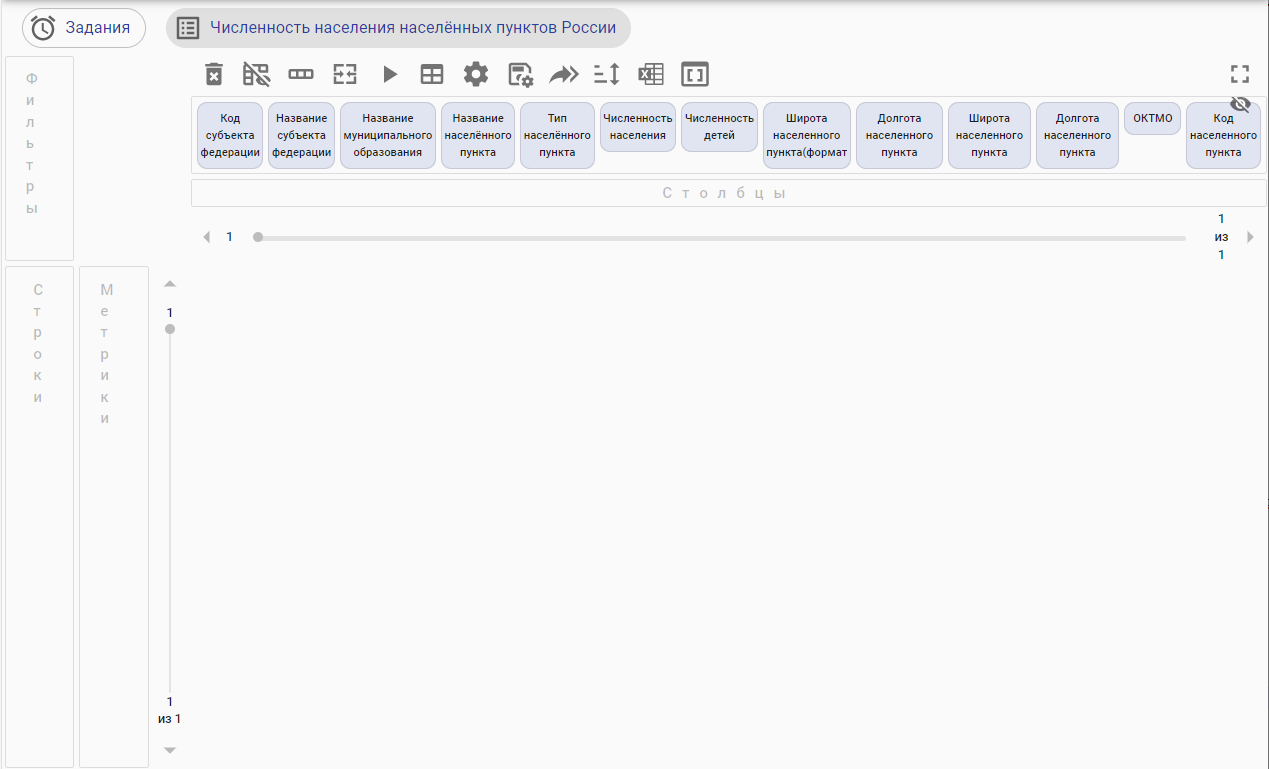
\includegraphics[width=\graphicswidth]{img/2-empty-pivot.png}
		\caption{Начальная конфигурация}
		\label{fig:empty-pivot}
	\end{figure}	

	Для получения разреза сводной таблицы, перетащите необходимые поля в области строк, столбцов и метрик, захватив их левой клавишей мыши.
	
	\begin{modelExample}
		В модельном примере создадим сводную в разрезе субъекта РФ и типа населенного пункта.		
		
		Поля отчета <<Код субъекта федерации>> и <<Название субъекта федерации>> поместим в область строк, а поле <<Тип населенного пункта>> в область столбцов.		
		
		В качестве метрик используем поля <<Численность населения>> и <<Численность детей>> с агрегатной функцией Сумма (см. рис. \ref{fig:pivot-01}).
	\end{modelExample}

	\begin{figure}[h]
		\centering
		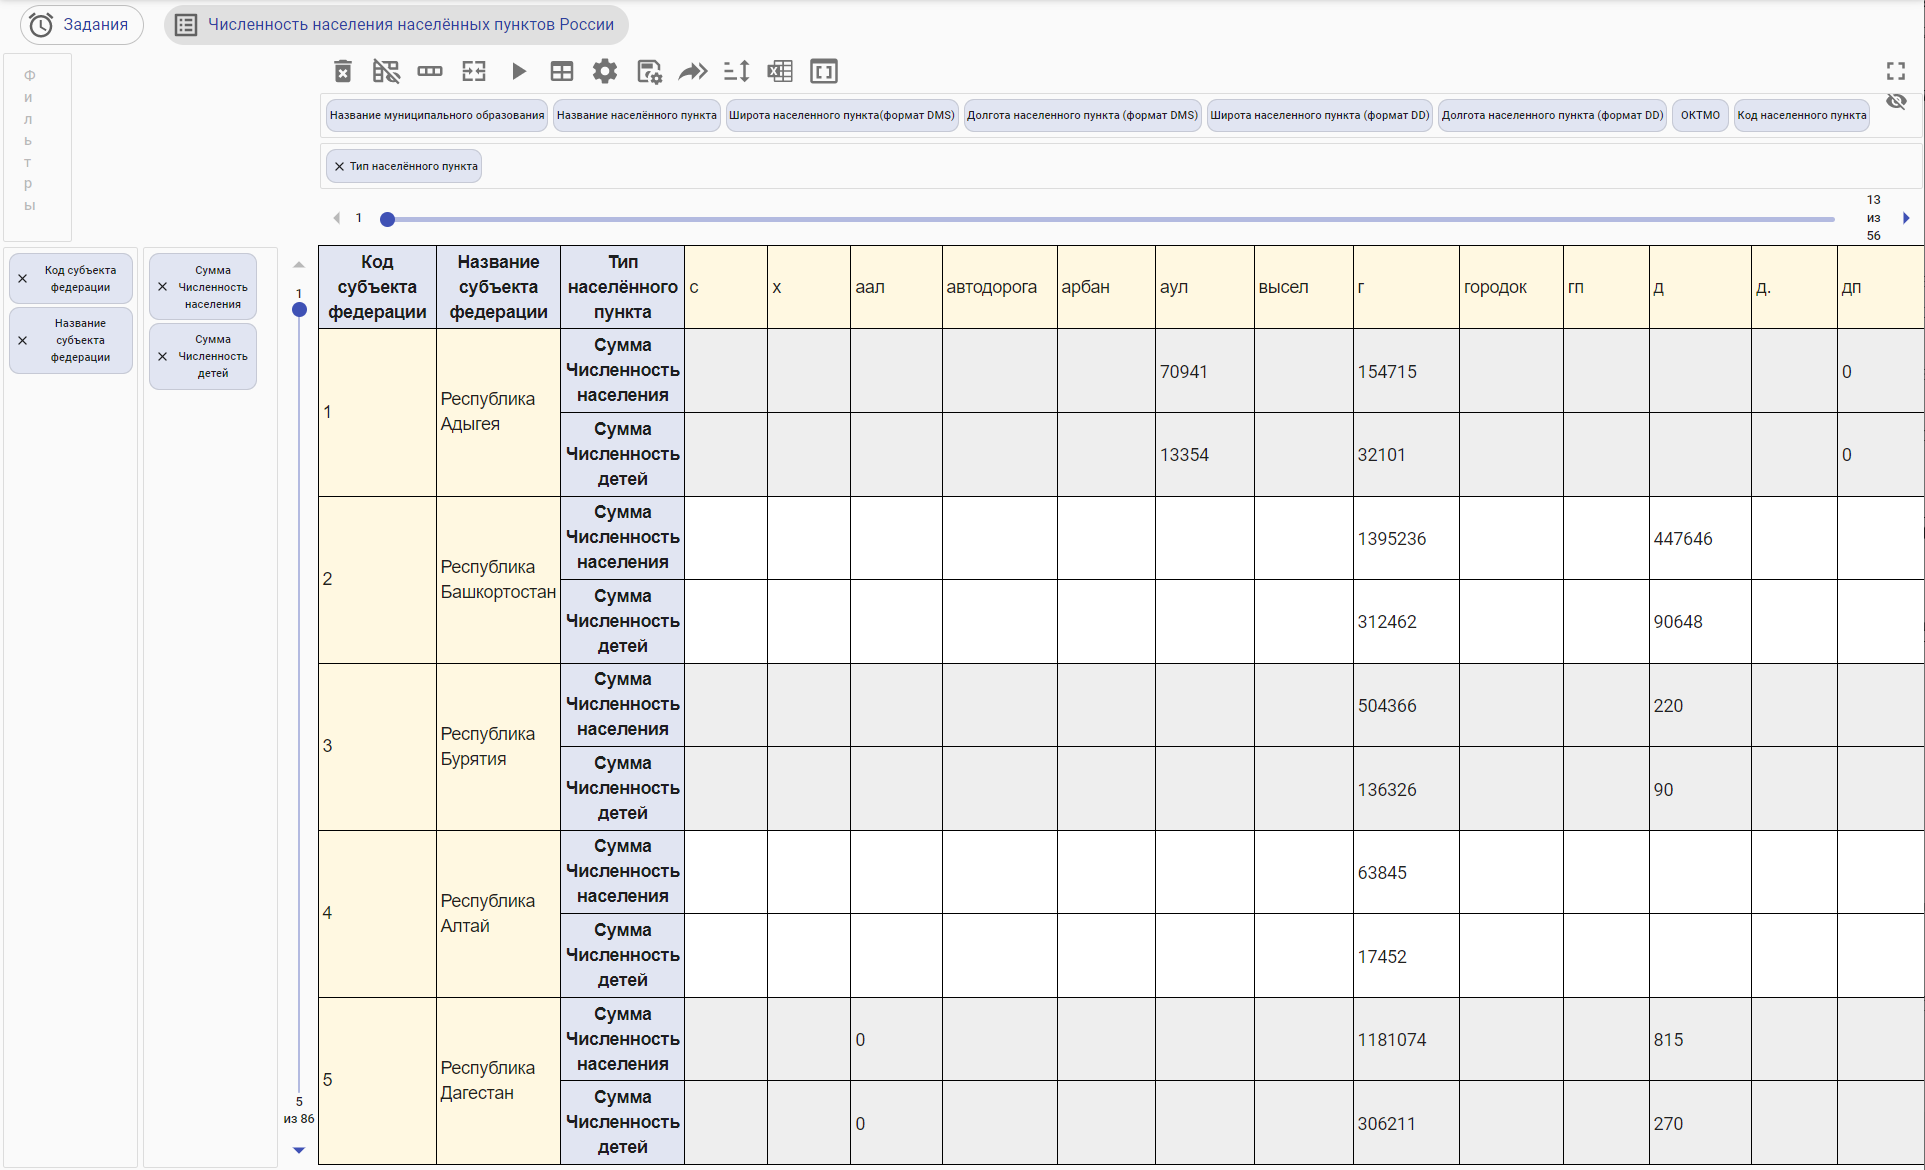
\includegraphics[width=\graphicswidth]{img/3-pivot-01.png}
		\caption{Вид сводной таблицы}
		\label{fig:pivot-01}
	\end{figure}	

	После помещения поля отчета в одну из областей сводной таблицы, это поле скрывается из области полей отчета.
	
	Для отображения всех полей отчета (включая используемые), необходимо нажать значок в верхнем правом углу области полей отчета (см. рис. \ref{fig:button-show-all}).
	
	\begin{figure}[h]
		\centering
		
\includegraphics[width=\graphicswidth]{img/4-show-all-but.png}
		\caption{Отображение всех полей}
		\label{fig:button-show-all}
	\end{figure}	

	Порядок полей в строках, столбцах и метриках изменяется захватом и перетаскиванием нужных полей левой клавишей мыши.
	
	Удаление поля из любой области сводной производится нажатием крестика в левом верхнем углу поля, подлежащего удалению.
	
	\begin{modelExample}
		В модельном примере удалим из области столбцов поле <<Тип населенного пункта>>.
	\end{modelExample}
	
	
	Для удобства отображения метрики могу располагаться как по строкам (см. рис. \ref{fig:metrics-on-string}), так и по столбцам (см. рис. \ref{fig:metrics-on-column}). 
	
	\begin{figure}[h]
		\centering
		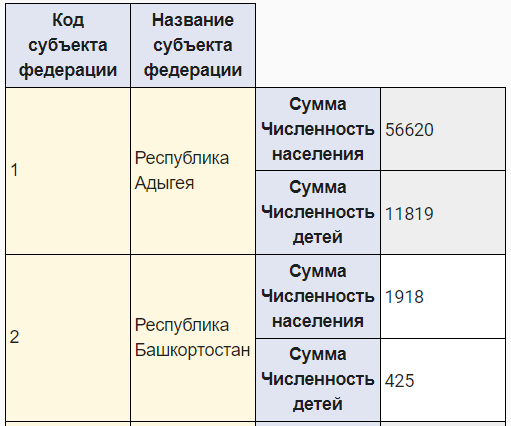
\includegraphics[width=\graphicswidth]{img/5-metrics-on-string.png}
		\caption{Метрики по строкам}
		\label{fig:metrics-on-string}
	\end{figure}

	\begin{figure}[h]
		\centering
		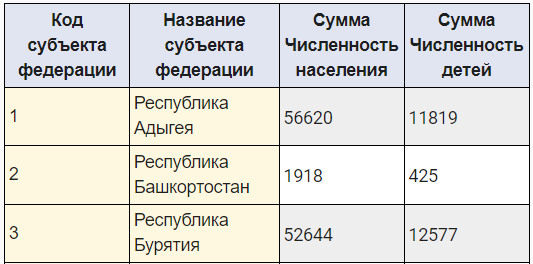
\includegraphics[width=\graphicswidth]{img/6-metrics-on-column.png}
		\caption{Метрики по столбцам}
		\label{fig:metrics-on-column}
	\end{figure}

	Можно изменить агрегирующую функцию, нажав правую клавишу мыши на нужной метрике.
	
	В зависимости от типа данных поля метрики, меняется перечень возможных агрегирующих функций.
	
	\begin{itemize}
		
		\item Для числовых полей доступны метрики:
			\begin{itemize}
				
				\item Сумма
				
				\item Количество
				
				\item Количество уникальных
				
				\item Минимальное значение
				
				\item Максимальное значение
				
				\item Среднее значение
			\end{itemize}
	
		\item Для строковых полей и полей типа дата доступны метрики:
			\begin{itemize}
			
				\item Количество
				
				\item Количество уникальных
			
				\item Минимальное значение
			
				\item Максимальное значение
			\end{itemize}
	
	\end{itemize}

	Чтобы изменить отображаемое название метрики, необходимо на метрике нажать левой клавишей мыши и ввести новое название в поле <<Описание>> (см. рис. \ref{fig:change-name}).
	
	\begin{figure}[h]
		\centering
		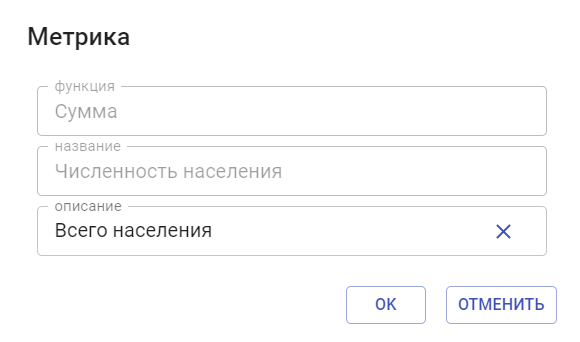
\includegraphics[width=\graphicswidth]{img/7-change-metrics-name.png}
		\caption{Изменение названия метрики}
		\label{fig:change-name}
	\end{figure}
	
	\section{Конфигурация сводной таблицы}
	
	Совокупность параметров представления сводной таблицы называется \textit{конфигурацией} сводной таблицы. То есть конфигурация полностью определяет, как именно данные будут отображены пользователю.
	
	Конфигурация сводной таблицы включает в себя следующие параметры:
	
	\begin{itemize}
				\item \textit{Строки} --- поля-измерения, расположенные по строкам сводной таблицы.
				
				\item \textit{Столбцы} --- поля-измерения, расположенные по столбцам сводной таблицы.
						
				\item \textit{Метрики} --- агрегируемые поля сводной таблицы.
			
				\item \textit{Фильтры} --- ограничивающие условия выводимых данных сводной таблицы.
			
				\item \textit{Сортировки} --- условия сортировки данных сводной таблицы.
			
				\item \textit{Форматирование} --- условное и безусловное форматирование полей метрик сводной таблицы.
				
				\item \textit{Начало диапазона просмотра} --- номер верхней строки и номер левого столбца сводной просматриваемого диапазона.
	\end{itemize}
	
	В конфигурацию не входит режим просмотра сводной --- полноэкранный или обычный. Также не входит режим отображения полей --- все или только не используемые. И не входит режим показа или сокрытия элементов управления конфигурацией.
	
	Конфигурации сводной можно сохранять, восстанавливать, делать общедоступными и ими можно делиться с другими пользователями (см. ниже).

	\section{Производные поля}
	
	\subsection{Работа с редактором производных полей}
	
	Помимо полей отчета в сводной таблице Магрепорт есть возможность использования производных полей, задаваемых при помощи встроенного языка формул Maglang.
	
	Для создания производных полей используется редактор, для открытия которого необходимо нажать кнопку <<Производные поля>> в меню сводной таблицы (см. рис. \ref{fig:derived_fields})
	
	\begin{figure}[h]
	\centering
	
\includegraphics[width=\graphicswidth]{img/30-derived_fields.png}
	\caption{Кнопка открытия редактора производных полей}
	\label{fig:derived_fields}
	\end{figure}

	В открывшемся окне (см. рис. \ref{fig:derived_fields_window}) показан список производных полей, доступных для отчета (область 1), кнопка создания нового производного поля, а также кнопки открытия справочника функций (3) и синтаксиса языка Maglang (4). Для удобства отображения можно изменить размер шрифта редактора (2).
	
	\begin{figure}[h]
	\centering
	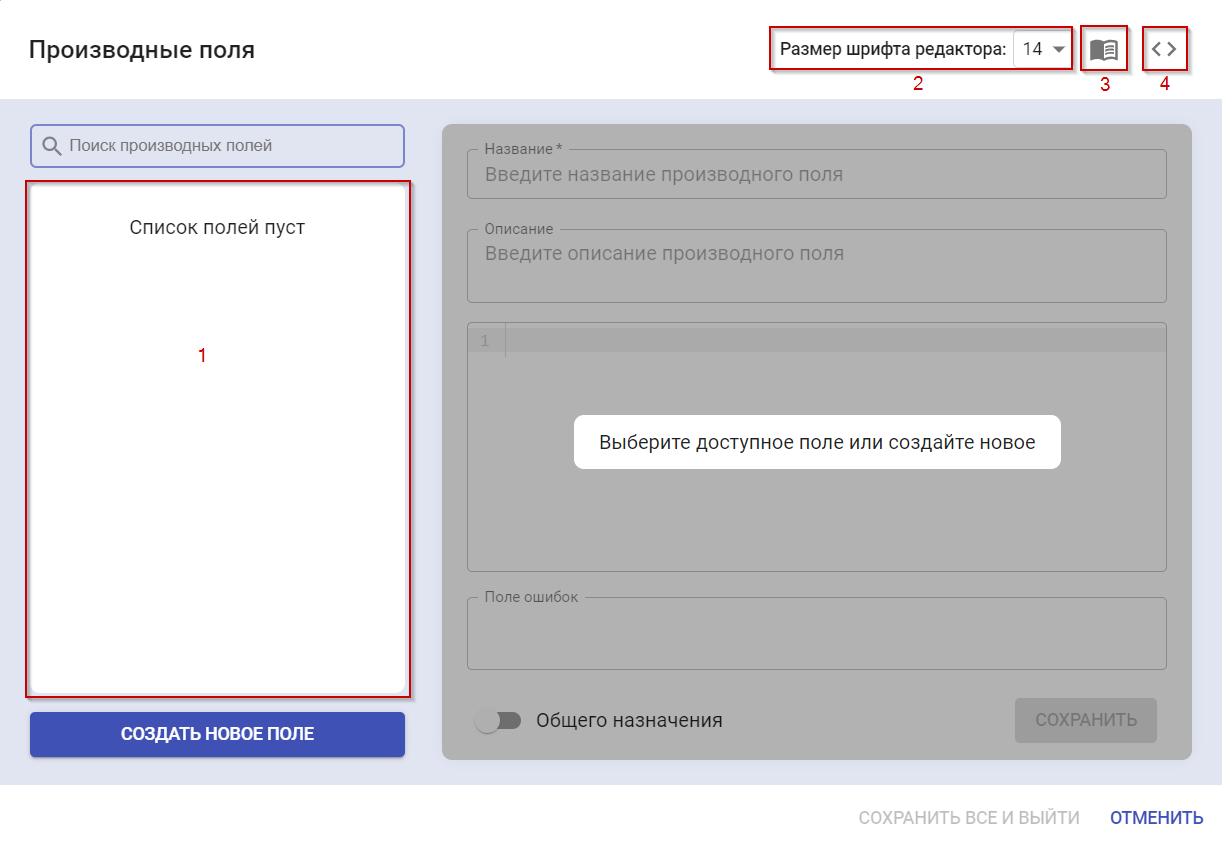
\includegraphics[width=\graphicswidth]{img/31-derived_fields_window.png}
	\caption{Окно редактора производных полей}
	\label{fig:derived_fields_window}
	\end{figure}

	Для создания нового поля необходимо нажать кнопку <<СОЗДАТЬ НОВОЕ ПОЛЕ>> и заполнить поля с названием и описанием поля, а также формулой. 
	
	Существующее поле можно редактировать, выбрав его в списке полей и изменив необходимые данные.
	
	Созданное производное поле будет появляться у пользователя во всех сводных таблицах, полученных из отчета, в котором это поле создано.
	
	Любое производное поле можно сделать общим, то есть можно поделиться таким полем с остальными пользователями Магрепорт, выставив переключатель <<Общего назначения>> (см. рис. \ref{fig:derived_fields_share}). 
	
	\begin{figure}[h]
		\centering
		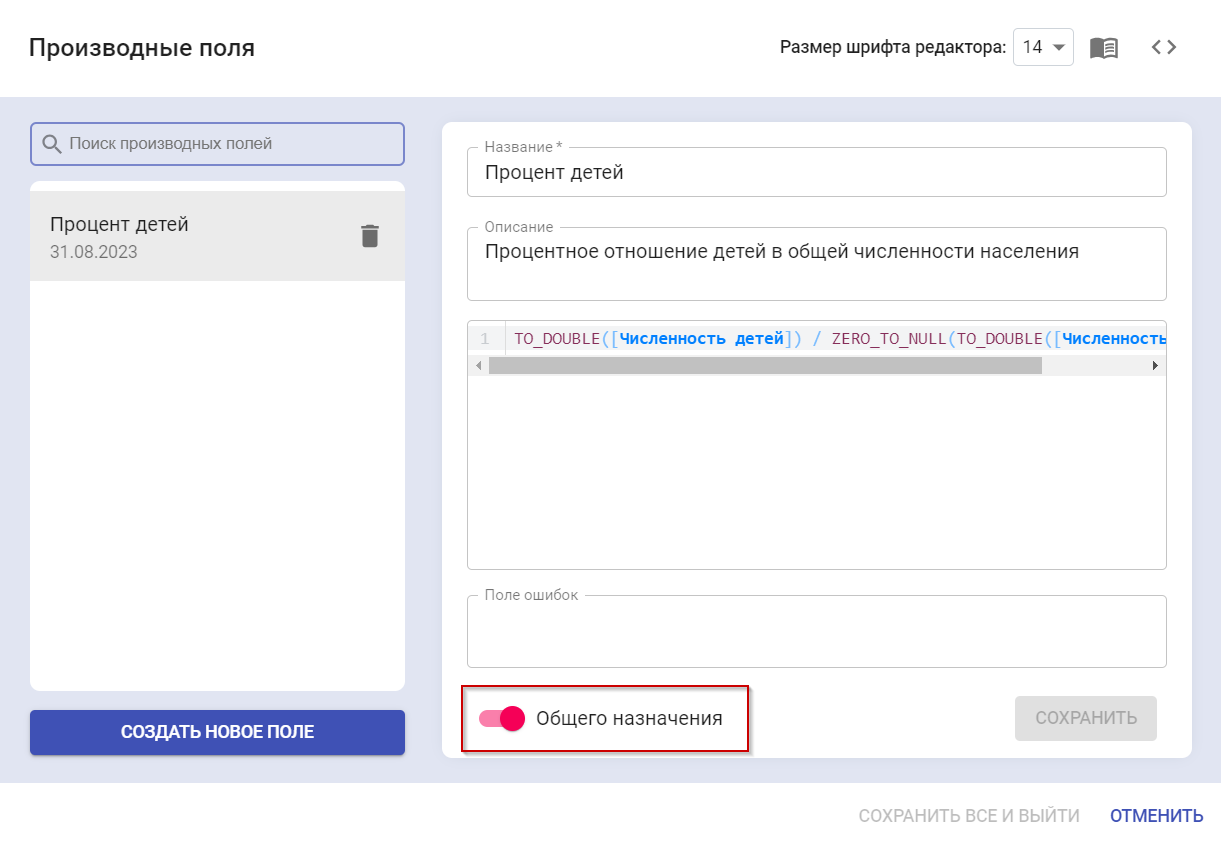
\includegraphics[width=\graphicswidth]{img/32-derived_fields_share.png}
		\caption{Создание общего производного поля}
		\label{fig:derived_fields_share}
	\end{figure}

	Названия производных полей отчета у пользователя должны быть уникальны. Однако, они могут совпадать с именами общих полей других пользователей. Более подробно о видимости и наименованиях производных полей можно прочитать в соответствующем разделе \ref{subsection:deriver-field-name}.
	
	\subsection{Синтаксис языка формул}	
	
	Язык формул Maglang позволяет задавать формулы для вычисления производных полей. Производные поля можно представлять себе, как вычисляемые столбцы, добавляемые в исходную таблицу сформированного набора данных отчета -- при этом в каждой строке в соответствующую ячейку столбца записывается значение, вычисленное по соответствующей формуле по значениям других ячеек в данной строке таблицы. 
	
	Для описания формул используются следующие языковые конструкции:
	\begin{itemize}
		
		\item \textbf{выражения} -- часть формулы, которая может быть вычислена как числовое, логическое, строковое значение или значение момента времени (даты или даты со временем); вся формула также представляет собой некоторое выражение;
		
		\item \textbf{константы} -- числовые, символьные и логические литералы; числовые литералы записываются в обычной форме записи с целой частью, дробной частью и экспонентой, нулевую целую часть можно опускать (3, -2.57, .18, 2E3, -3.5e4); целочисленные литералы представляются в системе через 64-битный целочисленный знаковый тип, вещественные -- через 64-битный тип чисел с плавающей запятой; символьные литералы записываются в виде строк, заключённых в двойные кавычки ("понедельник"); логически литералы записываются при помощи ключевых слов \textbf{True} и \textbf{False}; литералов для задания моментов времени (даты и даты со временем) не предусмотрено -- для их задания необходимо использовать соответствующие функции;
		
		\item \textbf{арифметические выражения} -- для числовых выражений доступно вычисление арифметических операций: сложение (+), вычитание (-), умножение (*), вещественное деление (/), целочисленное деление (то есть, целая часть от деления: //), вычисление остатка от деления (\%) и унарный минус (знак <<->> перед выражением); при вычислении арифметических выражений действуют обычные правила приоритета операций, для управления порядком вычислений можно использовать круглые скобки;
		
		\item \textbf{исходные поля отчёта} -- при вычислении выражений можно использовать значения полей, исходно присутствующих в отчёте, для этого, названия этих полей заключаются в одинарные квадратные скобки (например, [Продажи], [Потери], [Остаток]);
		
		\item \textbf{производные поля} -- при вычислении выражений можно использовать значения других производных полей (при этом главное, чтобы не было рекурсивных зависимостей в вычислениях), для этого, названия этих полей заключаются в двойные квадратные скобки (например, [[Маржинальность]], [[Относительные потери]]); имена производных полей, создаваемых конкретным пользователем обязаны быть уникальными, однако глобальная уникальность не требуется, также уникальными обязаны быть имена общедоступных производных полей -- производных полей, созданных разработчиком отчёта и объявленных, как общедоступные; при работе с производными полями пользователю доступны поля из текущей области видимости производных полей, которая включает в себя общедоступные производные поля, производные поля, созданные данным пользователем, и производные поля, присутствующие в данной конфигурации сводной таблицы; если в области видимости производных полей возникает дублирование имен, то более приоритетные поля остаются просто со своим именем, а к имени менее приоритетных через знак ";" (точка с запятой) добавляется логин пользователя, создавшего поле, приоритет полей от большего к меньшему: общедоступные производные поля, производные поля данного пользователя, производные поля других пользователей;
		
		\item \textbf{функции} -- при вычислении выражений могут использоваться функции из библиотеки функций, аргументами функций служат выражения, аргументы записываются через запятую;
		
		\item \textbf{условный оператор} -- условный оператор имеет вид:
		
		if(логическое выражение 1)\{
			выражение 1
		\}
		
		elif(логическое выражение 2)\{
			выражение 2
		\}
		
		elif(логическое выражение 3)\{
			выражение 3   
		\}
		
		...
		
		elif(логическое выражение N)\{
			выражение N
		\}
	
		else\{
			выражение по умолчанию
		\}
		
		при вычислении его возвращаемого значения происходит последовательное вычисление логических выражений вплоть до первого верного, при этом возвращается значение соответствующего выражения; если все условные выражения ложны -- возвращается значение выражения по умолчанию; блоки \textbf{elif} в условном операторе могут отсутствовать, блоки \textbf{if} и \textbf{else} обязательны;
		
		\item \textbf{логические выражения} -- логические выражения формируются при помощи операций сравнения и логических операций;
		
		\item \textbf{операции сравнения} -- стандартные операции меньше (<), больше (>), меньше либо равно (<=), больше либо равно (>=), равно (=), не равно (!= или <>);
		
		\item \textbf{логические операции} -- стандартные логические операции: логическое И (and), логическое ИЛИ (or), логическое ИСКЛЮЧАЮЩЕЕ ИЛИ (xor) и логическое ОТРИЦАНИЕ (not) -- последняя операция требует взятия в скобки инвертируемого логического выражения (например, <<not ([Продажи] < [Потери] and [Остаток] > 0)>>).
		
	\end{itemize}

	\begin{modelExample}
	В модельном примере создадим производное поле в сводной таблице, считающее процентную численность детей в общей численности населения региона.		
	
	
	Для этого в открывшемся окне работы с производными полями, необходимо нажать кнопку <<СОЗДАТЬ НОВОЕ ПОЛЕ>> и заполнить требуемые поля (см. рис. \ref{fig:derived-field}).
	
	В правом верхнем углу расположены кнопки для доступа к справочнику функций и синтаксису языка Maglang.
	
	
	Созданное производное поле появится в списке полей отчета (см. рис. \ref{fig:derived-field-2}). 
	
	Его можно добавить, как обычное поле: в строки, столбцы, метрики и фильтры (см. рис. \ref{fig:derived-field-3}).
	\end{modelExample}

	\begin{figure}[h]
		\centering
		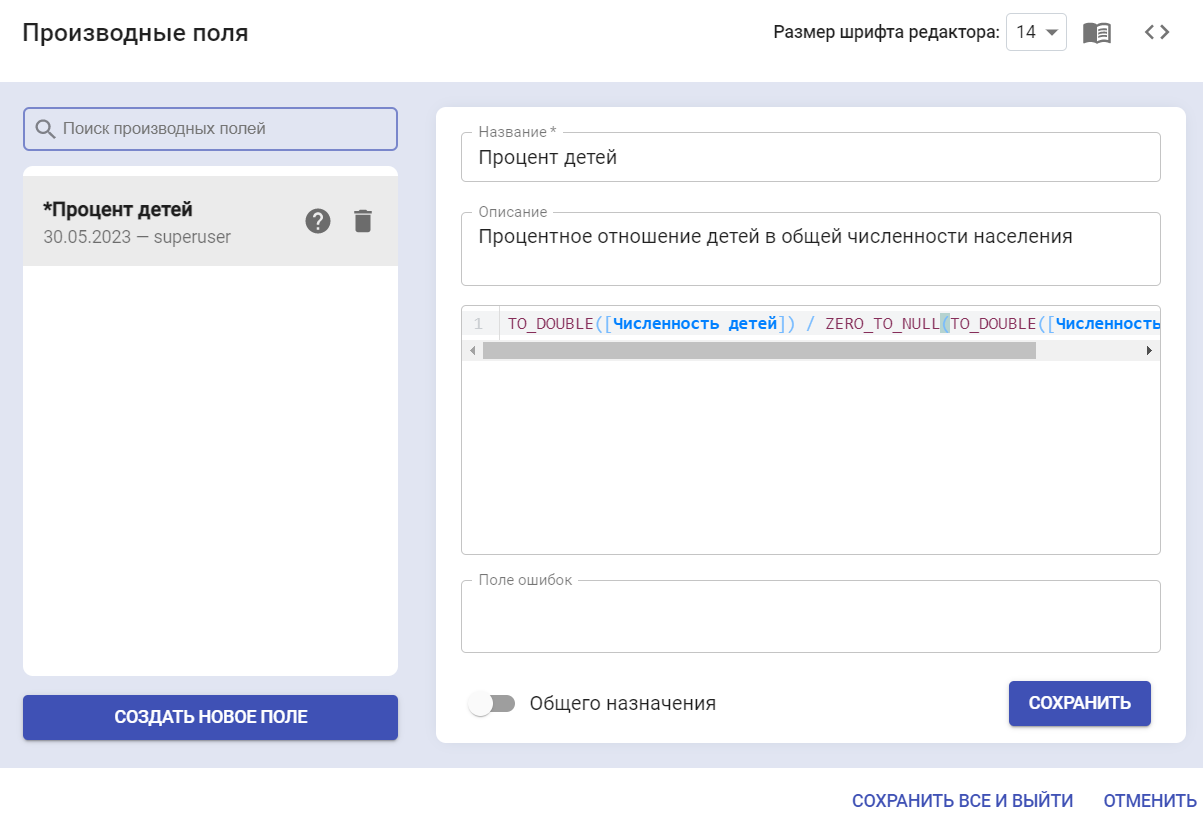
\includegraphics[width=\graphicswidth]{img/8-deriver-field.png}
		\caption{Создание производного поля}
		\label{fig:derived-field}
	\end{figure}

	\begin{figure}[h]
		\centering
		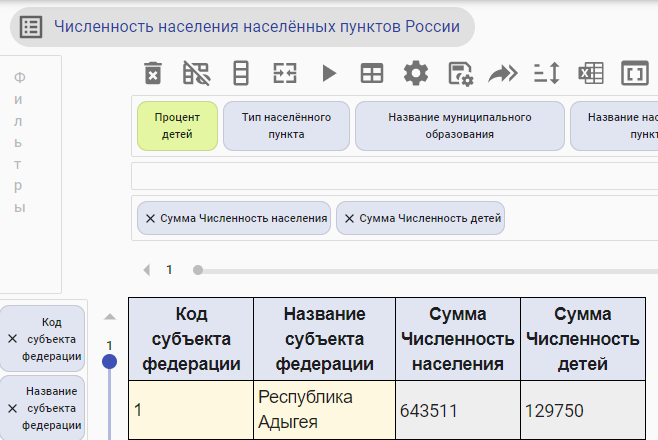
\includegraphics[width=\graphicswidth]{img/9-deriver-field.png}
		\caption{Производное поле в списке полей}
		\label{fig:derived-field-2}
	\end{figure}

	\begin{figure}[h]
		\centering
		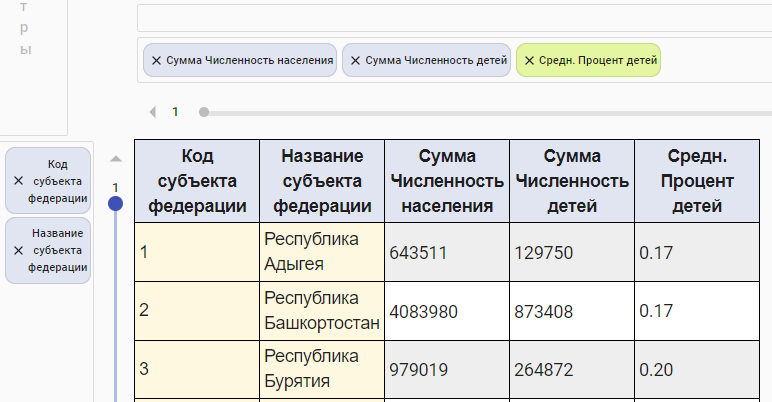
\includegraphics[width=\graphicswidth]{img/10-deriver-field.png}
		\caption{Производное поле в метриках}
		\label{fig:derived-field-3}
	\end{figure}
	
	\subsection{Видимость и наименование производных полей}\label{subsection:deriver-field-name}
	
	При работе со сводной таблицей и при редактировании производных полей пользователь видит поля, входящие в его \textit{зону видимости}. В зону видимости пользователя входят следующие производные поля:
	
	\begin{itemize}
		\item Производные поля, созданные пользователем (собственные поля пользователя).
		
		\item Общедоступные производные поля (поля общего назначения).
		
		\item Производные поля, созданные другими пользователями, но присутствующие в текущей конфигурации.
		
	\end{itemize}
	
	На производные поля, созданные одним и тем же пользователем, накладывается требования уникальности имён. Поля, созданные разными пользователями, могут иметь одинаковые имена. Также наклывается требование уникальности имени на общедоступные производные поля.
	
	При использовании производных полей пользователь видит \textit{локальное именование} производного поля. Локальные именования производных полей строятся таким образом, чтобы они образовывали совокупность уникальных имён, так как при написании формул языка обращение к производным полям происходит по их имени. Локальные имена производных полей формируются следующим образом:
	
	\begin{itemize}
		
		\item У производных поля общего назначения локальное имя совпадает с его именем.
		
		\item У производных полей, владельцем которых является данный пользователь локальное имя совпадает с его именем, если оно не встречается среди имён полей общего назначения, иначе к имени в конце добавляется логин пользователя в скобках.
		
		\item У производных полей, не являющихся полями общего назначения, владельцем которых является другой пользователь, локальное имя совпадает с его именем, если такое имя не встречается среди полей общего назначения и собственных полей данного пользователя, иначе к имени добавляется логин пользователя-владельца в скобках.
		
	\end{itemize}
	
	Например, пользователь petrov поделился с пользователем ivanov выполненным отчётом по продажам, в котором есть общедоступное поле \textit{Маржинальность} и поле \textit{Маржинальность}, созданное пользователем petrov и присутствующее в данной конфигурации. Кроме того, у пользователя petrov в этой конфигурации есть ещё производные поля \textit{Относительные потери} и \textit{Категория по выручке}. У пользователя ivanov есть собственные производные поля \textit{Маржинальность} и \textit{Относительные потери}, общедоступного поля с именем \textit{Относительные потери} не существует. Пользователь ivanov при работе с данной конфигурацией будет видеть следующие локальные наименования производных полей:
	
	\begin{tabular}{l}
		
		Маржинальность\\
		
		Маржинальность(ivanov)\\
		
		Маржинальность(petrov)\\
		
		Относительные потери\\
		
		Относительные потери(petrov)\\
		
		Категория по выручке\\
		
	\end{tabular}
	
	
	\section{Форматирование сводной таблицы}
	
	Для удобства отображения данных в сводной таблице Магрепорт есть возможность безусловного и условного форматирования.
	
	\subsection{Безусловное форматирование}
	
	Безусловное форматирование полей, содержащих числа, позволяет задать формат значений метрик (рис. \ref{fig:format-number}):
	\begin{itemize}
		
		\item количество знаков после запятой
		
		\item процентный вид
		
		\item разрядный вид
	\end{itemize}

	Безусловное форматирование полей, содержащих строки, позволяет задать количество отображаемых символов (рис. \ref{fig:format-string}).
	
	Также есть возможность выделить определенные метрики (рис. \ref{fig:format-font}):
	\begin{itemize}
	
		\item начертанием шрифта (жирный, курсив, подчеркнутый)
	
		\item размером шрифта
	
		\item цветом шрифта
	\end{itemize}
	\begin{figure}[h!]
		\centering
		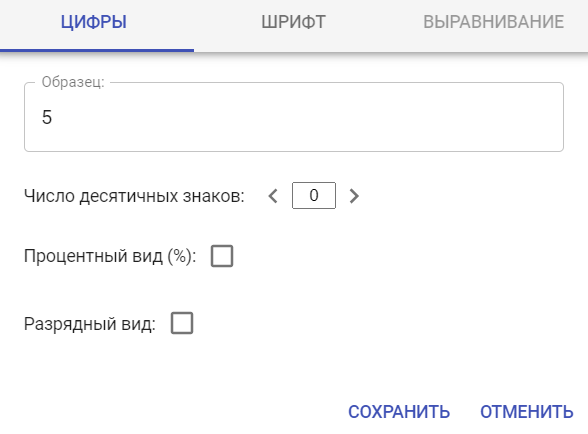
\includegraphics[width=\graphicswidth]{img/11-format-number.png}
		\caption{Безусловное форматирование чисел}
		\label{fig:format-number}
	\end{figure}
	\begin{figure}[h!]
		\centering
		
\includegraphics[width=\graphicswidth]{img/12-format-string.png}
		\caption{Безусловное форматирование строк}
		\label{fig:format-string}
	\end{figure}
	\begin{figure}[h!]
		\centering
		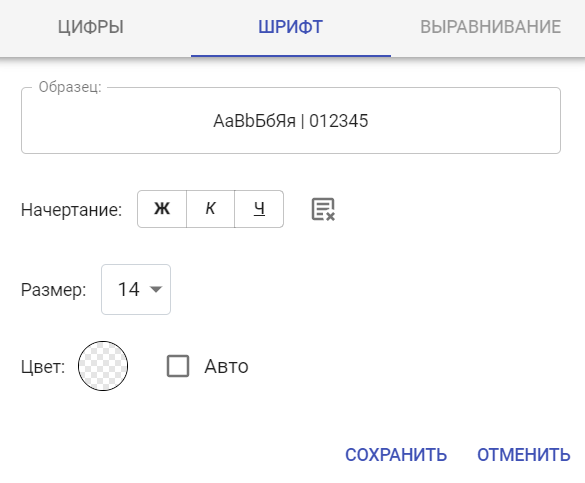
\includegraphics[width=\graphicswidth]{img/13-format-font.png}
		\caption{Задание вида шрифта метрики}
		\label{fig:format-font}
	\end{figure}
	
	\begin{modelExample}
		В модельном примере отформатируем поле <<Процент детей>>.
		
		Для этого на любой ячейке со значением поля нажмем правой кнопкой мыши и выберем из контекстного меню пункт <<Форматирование>> (рис. \ref{fig:format-example-1}).

		В появившемся меню выставляем <<Процентный вид>>, выбираем цвет шрифта и жирное начертание.
		
		Результат безусловного форматирования представлен на рисунке \ref{fig:format-example-2}
	\end{modelExample}

	\begin{figure}[h]
		\centering
		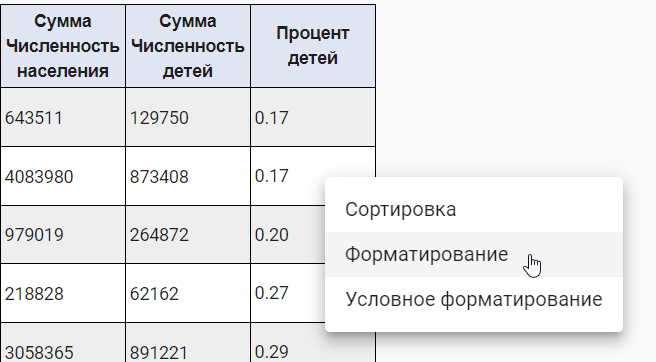
\includegraphics[width=\graphicswidth]{img/14-format-example.png}
		\caption{Контекстное меню ячеек сводной}
		\label{fig:format-example-1}
	\end{figure}

	\begin{figure}[h]
		\centering
		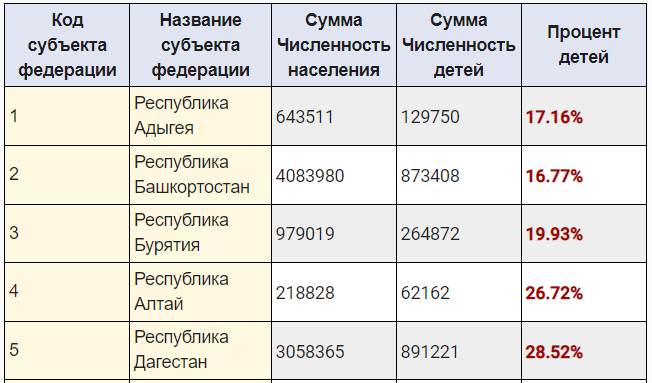
\includegraphics[width=\graphicswidth]{img/16-format-example.png}
		\caption{Безусловное форматирование ячеек}
		\label{fig:format-example-2}
	\end{figure}
	
	\subsection{Уусловное форматирование}

	Условное форматирование позволяет визуально разделить данные полей по их значениям.
	
	Магрепорт позволяет сформировать до 10 непрерывных периодов значений полей, для каждого из которых можно задать формат значений метрик (цвет фона, цвет и размер шрифта, стиль начертания).
	
	Для этого на любой ячейке со значением метрики, для которой требуется условное форматирование, нажать правой клавишей мыши и выбрать в меню <<Условное форматирование>> (рис. \ref{fig:format-example-1}).
	
	В открывшемся окне  (рис. \ref{fig:conditional-format-1}) нажать кнопку <<Разделить>> столько раз, сколько необходимо, чтобы получить требуемое количество диапазонов значений.
	
	\begin{figure}[h]
		\centering
		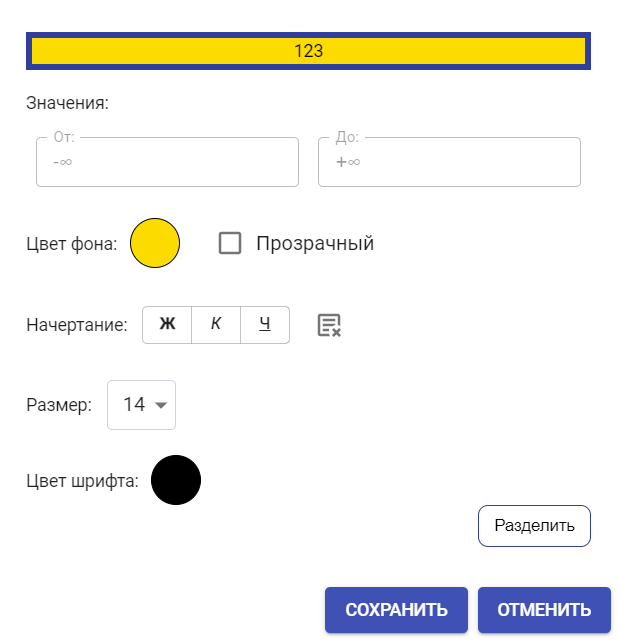
\includegraphics[width=\graphicswidth]{img/17-conditional-format.png}
		\caption{Условное форматирование метрик}
		\label{fig:conditional-format-1}
	\end{figure}
	
		
	Для каждого диапазона необходимо указать начальное и конечное значение (при указании конечного значения диапазона, начальное значение следующего за ним диапазона становится равным введенному, диапазоны считаются открытыми справа и закрытыми слева, то есть если, например, число 1000 разграничивает два диапазона, то значения строго меньше 1000 попадают в левый диапазон, а 1000 и больше~--- в правый).
	
	Переключаясь между диапазонами, можно выбрать формат значений метрики, попадающих в данный диапазон.
		
	\begin{modelExample}
		В модельном примере сделаем условное форматирования поля <<Процент детей>> по следующему сценарию:
		
		\begin{itemize}
			\item при значении до 20\% ячейки выделить желтым цветом
			\item при значении от 20\% до 30\% -- голубым
			\item больше 30\% -- зеленым.
		\end{itemize}
	
		Для этого на любой ячейке со значением поля нажмем правой кнопкой мыши и выберем из контекстного меню <<Условное форматирование>>.
		
		В открывшемся окне дважды нажать кнопку <<Разделить>>.
		
		Переключаясь между диапазонами установить требуемые значения и цвет ячеек (пример среднего диапазона показан на рис. \ref{fig:conditional-format-2}).
		
		Аналогично сделаем условное форматирование метрики <<Численность населения>>:
		
		\begin{itemize}
			\item при численности до 1 000 000 человек -- выделить ячейку фиолетовым цветом,
			\item свыше 1 000 000 -- розовым.
		\end{itemize}
		
		Результат условного форматирования представлен на рисунке \ref{fig:conditional-format-3}
	\end{modelExample}

	\begin{figure}[h]
		\centering
		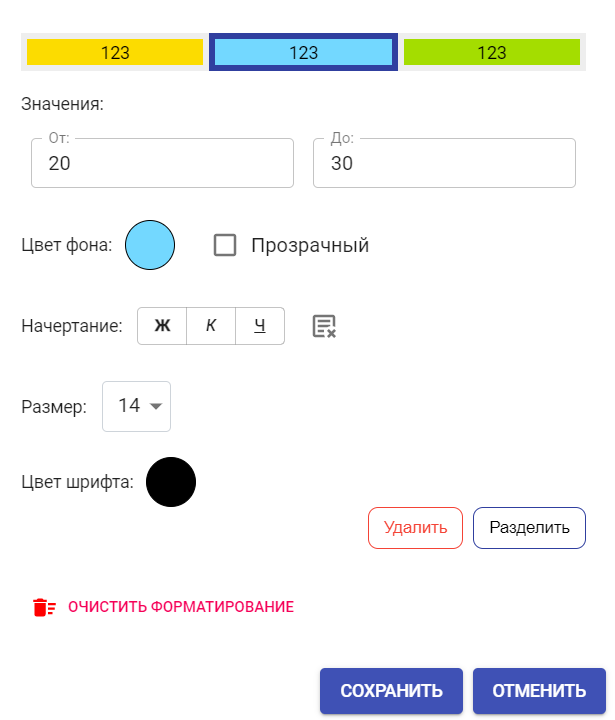
\includegraphics[width=\graphicswidth]{img/18-conditional-format.png}
		\caption{Меню условного форматирование метрик}
		\label{fig:conditional-format-2}
	\end{figure}

	\begin{figure}[h]
		\centering
		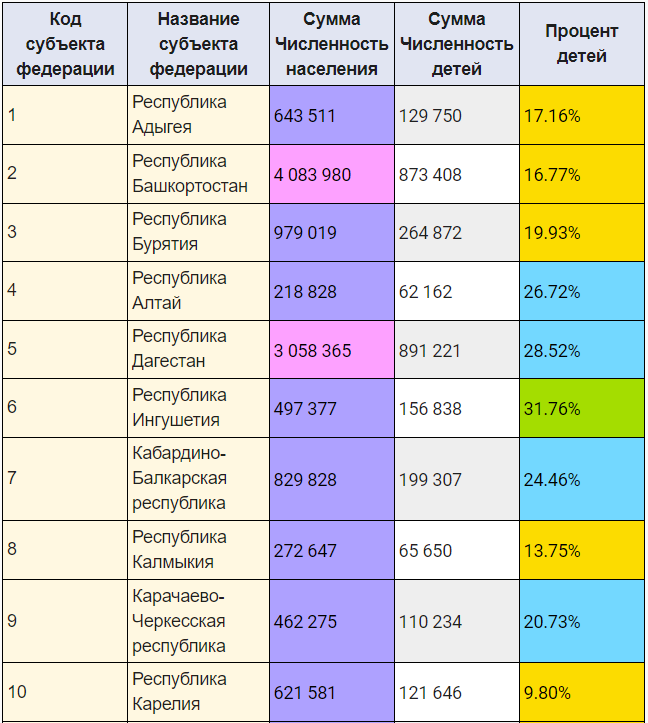
\includegraphics[width=\graphicswidth]{img/19-conditional-format.png}
		\caption{Результат условного форматирования}
		\label{fig:conditional-format-3}
	\end{figure}


	\section{Фильтры в сводной таблице}
	
	Магрепорт позволяет отфильтровать данные отчета по разным параметрам. Фильтрация осуществляется как по полям отчета, используемым в сводной таблице, так и по другим полям отчета, которые не находятся в областях строк, столбцов и метрик.
	
	Фильтрация применяется к исходному набору данных до агрегации. Действие фильтров аналогично действию предиката SQL-запроса в секции WHERE. 
	
	Аналогично агрегирующим функциям для метрик, у полей разных типов данных могут быть разные варианты фильтров.

	Для числовых полей возможны следующие параметры фильтрации:
	
	\begin{itemize}
		
		\item \textbf{Равно / НЕ Равно} -- оставляет в сводной таблице строки, где выбранное поле равно (не равно) определенному значению;
		
		\item \textbf{Больше / НЕ Больше} -- оставляет строки, где поле больше (не больше) определенного значения;
		
		\item \textbf{Меньше / НЕ Меньше} -- оставляет строки, где поле меньше (не меньше) определенного значения;
		
		\item \textbf{Больше или равно / НЕ Больше или равно} -- оставляет строки, где поле больше или равно (не больше или равно) определенному значению;
		
		\item \textbf{Меньше или равно / НЕ Меньше или равно} -- оставляет строки, где поле меньше или равно (не меньше или равно) определенному значению;
		
		\item \textbf{Между (включительно) / НЕ Между (включительно)} -- оставляет строки, где значение поля находится между (вне) двух определенных значений;
		
		\item \textbf{Пусто / НЕ Пусто} -- оставляет строки, где поле пустое (не пустое).
		
	\end{itemize}
	
	Для текстовых полей и полей типа дата возможны следующие параметры фильтрации:
	
	\begin{itemize}
		
		\item \textbf{Равно / НЕ Равно} -- оставляет в сводной таблице строки, где выбранное поле равно (не равно) определенному значению;
		
		\item \textbf{В списке / НЕ В списке} -- оставляет строки, где значение поля входит (не входит) в список выбранных значений;
		
		\item \textbf{Содержит (без учета регистра) / НЕ Содержит (без учета регистра)} -- оставляет строки, где поле содержит (не содержит) определенную подстроку без учета регистра;
		
		\item \textbf{Содержит (с учетом регистра) / НЕ Содержит (с учетом регистра)} -- оставляет строки, где поле содержит (не содержит) определенную подстроку с учетом регистра;
		
		\item \textbf{Пусто / НЕ Пусто} -- оставляет строки, где поле пустое (не пустое).
		
	Удобным способом фильтрации данных в сводной Магрепорт является нажатие левой клавишей мыши на значение ячейки сводной таблицы. При этом формируется фильтр по полю выбранной ячейки с условием фильтрации <<Равно>> выбранному значению.
		
	\end{itemize}

	\begin{modelExample}
		В модельном примере оставим строки, где численность населения в регионе превышает 1 млн. чел.
	
		Для этого на любой ячейке со значением поля <<Численность населения>> нажмем левой клавишей мыши.
	
		В области фильтров появится это поле. Нажатие на него левой клавишей мыши, приведет к открытию меню выбора условия фильтрации.
	
		В выпадающем меню выберем пункт <<Больше>> (рис. \ref{fig:filtration-menu-1}). В поле значений введем 1000000.
	
		Также оставим только регионы, являющиеся республиками. Для этого захватим поле <<Название субъекта федерации>> (в области всех полей отчета или области строк) левой клавишей мыши и перетащим в область фильтров. В открывшемся меню выберем пункт <<Содержит (без учета регистра)>>, а в поле значения введем <<республика>>.

		Результат фильтрации представлен на рисунке \ref{fig:filtered-pivot}
	\end{modelExample}

	\begin{figure}[h]
		\centering
		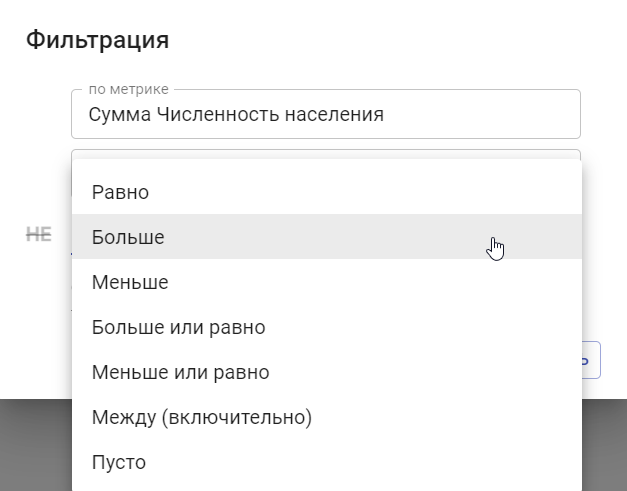
\includegraphics[width=\graphicswidth]{img/20-filtration_menu.png}
		\caption{Меню фильтра}
		\label{fig:filtration-menu-1}
	\end{figure}

	\begin{figure}[h]
		\centering
		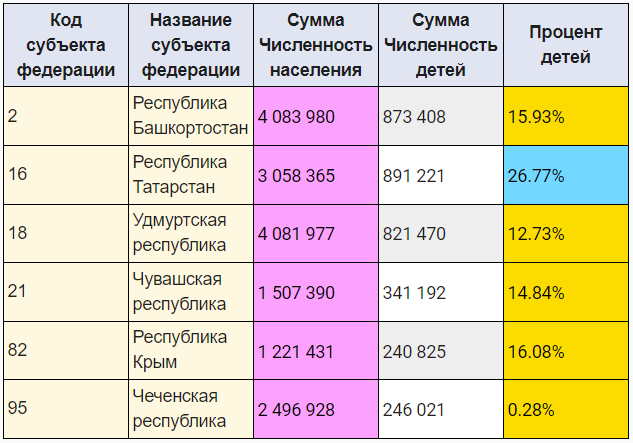
\includegraphics[width=\graphicswidth]{img/21-filtered-pivot.png}
		\caption{Отфильтрованная сводная таблица}
		\label{fig:filtered-pivot}
	\end{figure}

	Для изменения значения или условия фильтрации существующего фильтра на таком фильтре необходимо нажать левой клавишей мыши.
	
	Для удаления фильтра~--- нажать крестик в левой части фильтра.
	
	Ненужный в данный момент фильтр можно отключить, не удаляя. Для этого на таком фильтре необходимо нажать правой клавишей мыши. При этом деактивированный фильтр становится серым. Для повторной активации фильтра также необходимо нажать на нем правой клавишей мыши.
	
	Часть сводной таблицы из модельного примера с отключенным фильтром по численности населения представлен на рисунке \ref{fig:filter-example}.
	
	\begin{figure}[h]
		\centering
		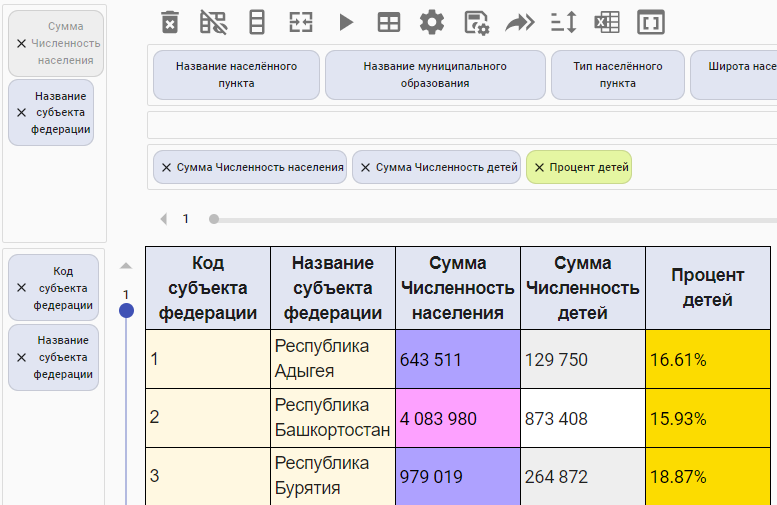
\includegraphics[width=\graphicswidth]{img/22-filter-exam.png}
		\caption{Пример сводной таблицы с фильтрами}
		\label{fig:filter-example}
	\end{figure}
	
	При использовании условия фильтрации <<В списке>> необходимые значения поля переносятся в область значений фильтра их выделением слева и нажатием кнопки переноса их в правую часть окна (см. рис. \ref{fig:filter-list}). В левой части окна можно регулировать количество отображаемых значений на странице и переключаться между страницами со значениями. Обратите внимание, что выделение значений слева без переноса в правую часть не является заданием значений для фильтрации. В фильтре будут использованы только значения, расположенные в правой части окна выбора значений фильтра.
		
	\begin{figure}[h]
		\centering
		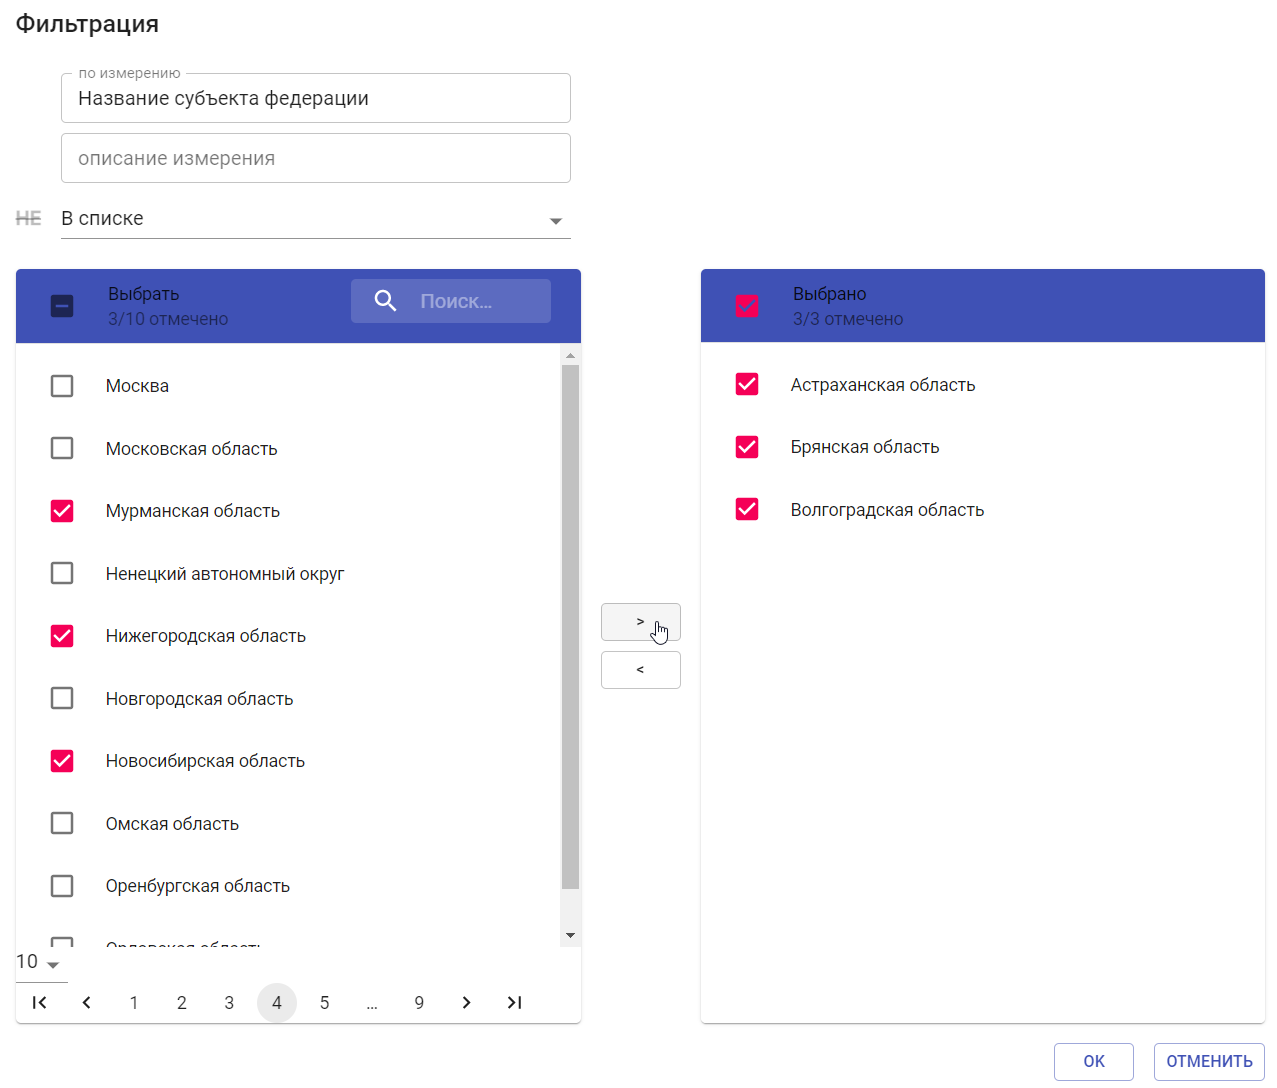
\includegraphics[width=\graphicswidth]{img/23-filter-list.png}
		\caption{Фильтр <<В списке>>}
		\label{fig:filter-list}
	\end{figure}

	
	\section{Сортировка сводной таблицы}
	
	В Магрепорт возможна сортировка данных сводной таблицы как по столбцам, так и по строкам метрик.
	
	При наведении на ячейку метрики проявляются стрелки сортировки (см. рис. \ref{fig:sort-button}). При нажатии на соответствующую стрелочку, будет произведена сортировка в направлении нажатой стрелочки относительно выбранной ячейки.
	
	\begin{figure}[h]
		\centering
		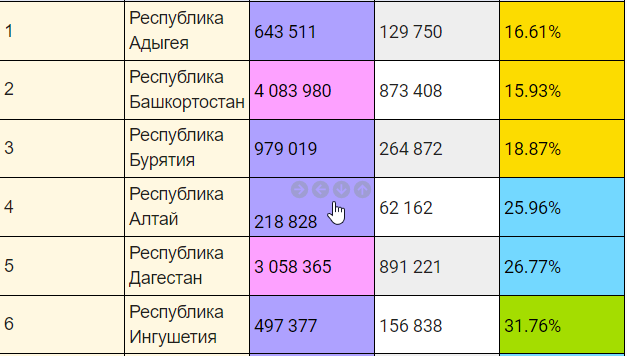
\includegraphics[width=\graphicswidth]{img/24-sort-button.png}
		\caption{Кнопки для сортировки метрик}
		\label{fig:sort-button}
	\end{figure}

	\begin{modelExample}
		В модельном примере отсортируем данные в порядке уменьшения процента детей в регионе.
		
		После нажатия стрелочки, указывающей вверх на любой ячейке со значением поля <<Процент детей>>, получится отсортированная сводная, часть которой показана на рисунке \ref{fig:sorted-pivot}. 
		
		Зеленые стрелочки в ячейках метрики показывают направление увеличение значений.
	
	\end{modelExample}

	\begin{figure}[h]
		\centering
		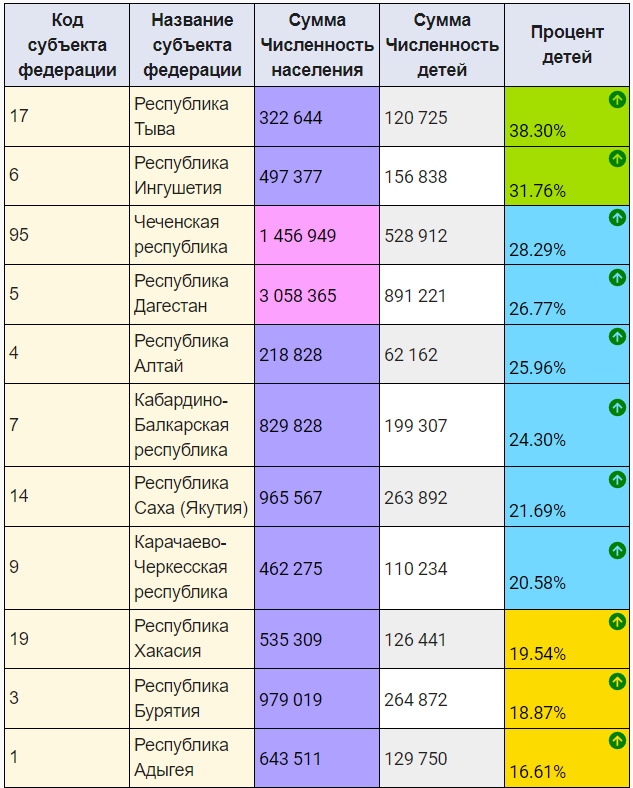
\includegraphics[width=\graphicswidth]{img/25-sort-pivot.png}
		\caption{Отсортированная по полю <<Процент детей>> сводная таблица}
		\label{fig:sorted-pivot}
	\end{figure}
	
		
	\section{Сохранение и использование конфигураций сводной таблицы отчета}
	
	Конфигурация, в котором пользователю в данный момент отображается сводная таблица, называется \textit{текущей конфигурацией}. При любом действии пользователя, приводящем к изменению текущей конфигурации сводной она автоматически сохраняется на сервере. При завершении работы с данным выполненным отчётом и при последующем входе в этот же отчёт пользователю автоматически загружается последняя теукщая конфигурация и сводная представляется в соответствующем виде.
	
	Текущую конфигурацию сводной таблицы можно сохранить для дальнейшего использования.
	
	Варианты сохранения конфигурации:
	
	\begin{itemize}
		
		\item \textbf{для задания} -- сохраненная конфигурация будет доступна пользователю только для этого задания;
		
		\item \textbf{для отчета} -- сохраненная конфигурация будет доступна пользователю во всех заданиях текущего отчета;
		
		\item \textbf{для всех} -- вариант сохранения доступен для разработчика отчета -- сохраненная конфигурация будет видна всем пользователям, имеющим доступ к отчету (данная опция сохранения доступна только пользователям, обладающим правами разработчика данного отчёта).
		
	\end{itemize}

	Конфигурации, сохраненные <<для отчета>> или <<для всех>>, могут быть установлены в качестве конфигурации по умолчанию. Тогда при открытии сводной таблицы нового задания отчета, будет загружена конфигурация, установленная по умолчанию.
	
	При открытии сводной таблицы выполненного отчёта действуют следующие правила выбора конфигурации, в которой выполняется представление сводной:
	
	\begin{itemize}
		
		\item Если пользователь ранее уже работал с этим заданием в сводной, сводная открывается в текущей конфигурации.
		
		\item Иначе, если пользователь не является владельцем данного задания (с ним данным заданием поделились), сводная открывается в той конфигурации, в которой она была представлена в момент, когда с данным пользователем поделились данным заданием.
		
		\item Иначе, если у пользователя установлена собственная конфигурация сводной для данного отчёта по умолчанию, сводная открывается в этой конфигурации.
		
		\item Иначе, если для данного отчёта разработчиком задана конфигурация сводной по умолчанию для всех пользователей, сводная открывается в этой конфигурации.
		
		\item Иначе, сводная открывается в пустой конфигурации.
		
	\end{itemize}
	
	К конфигурациям, сохраненным <<для задания>>, можно предоставить доступ другим пользователям. Такие конфигурации доступны для выбора всеми пользователями, которым доступно данное задание (с которыми поделились этим заданием или которые получили его в резальтате выполнения отчёта по расписанию).
	
	Для сохранения новой конфигурации или перезаписи существующей необходимо нажать в меню кнопку <<Сохранить конфигурацию>> (см. рис. \ref{fig:pivot-menu}).
	
	В открывшемся окне (рис. \ref{fig:save-pivot}) необходимо ввести название и описание конфигурации (при сохранении новой) или перейти на вкладку <<Существующие конфигурации>> и выбрать из выпадающего списка ту, которую надо заменить.
	
	\begin{figure}[h]
		\centering
		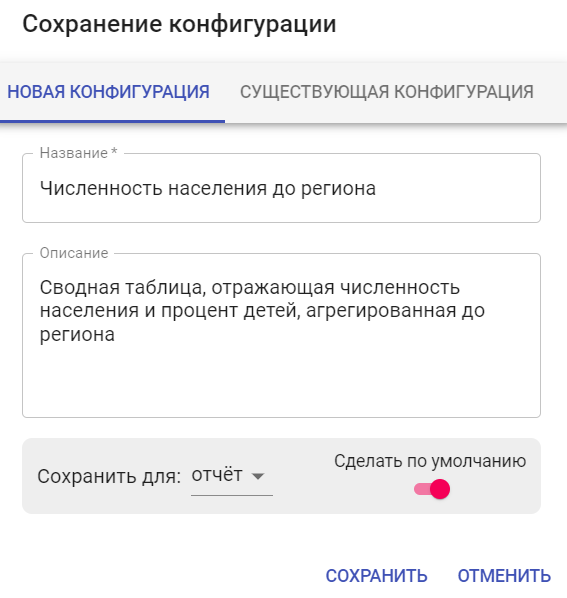
\includegraphics[width=\graphicswidth]{img/26-save-pivot.png}
		\caption{Сохранение текущей конфигурации}
		\label{fig:save-pivot}
	\end{figure}	
	
	
	\begin{modelExample}
		
		В модельном примере сохраним текущую конфигурацию для отчета с отметкой по умолчанию.
		
		При просмотре существующих конфигураций (кнопка 7 рис. \ref{fig:pivot-menu}) появится сохраненная выше конфигурация (см. рис. \ref{fig:config-list}). 
				
	\end{modelExample}

	\begin{figure}[h]
		\centering
		
\includegraphics[width=\graphicswidth]{img/27-config-list.png}
		\caption{Доступные конфигурации}
		\label{fig:config-list}
	\end{figure}	
		
	
	\section{Предоставление конфигурации другим пользователям}
		
	Любой текущей конфигурацией сводной можно поделиться с другим пользователем Магрепорт.
	
	Для этого надо нажать на кнопку <<Поделиться заданием>> в меню сводной таблицы (кнопка 9 рис. \ref{fig:pivot-menu}).
	
	В открывшемся окне отметить пользователей, которым необходимо предоставить доступ к текущей конфигурации (см. рис. \ref{fig:share-pivot}).
	
	\begin{figure}[h]
		\centering
		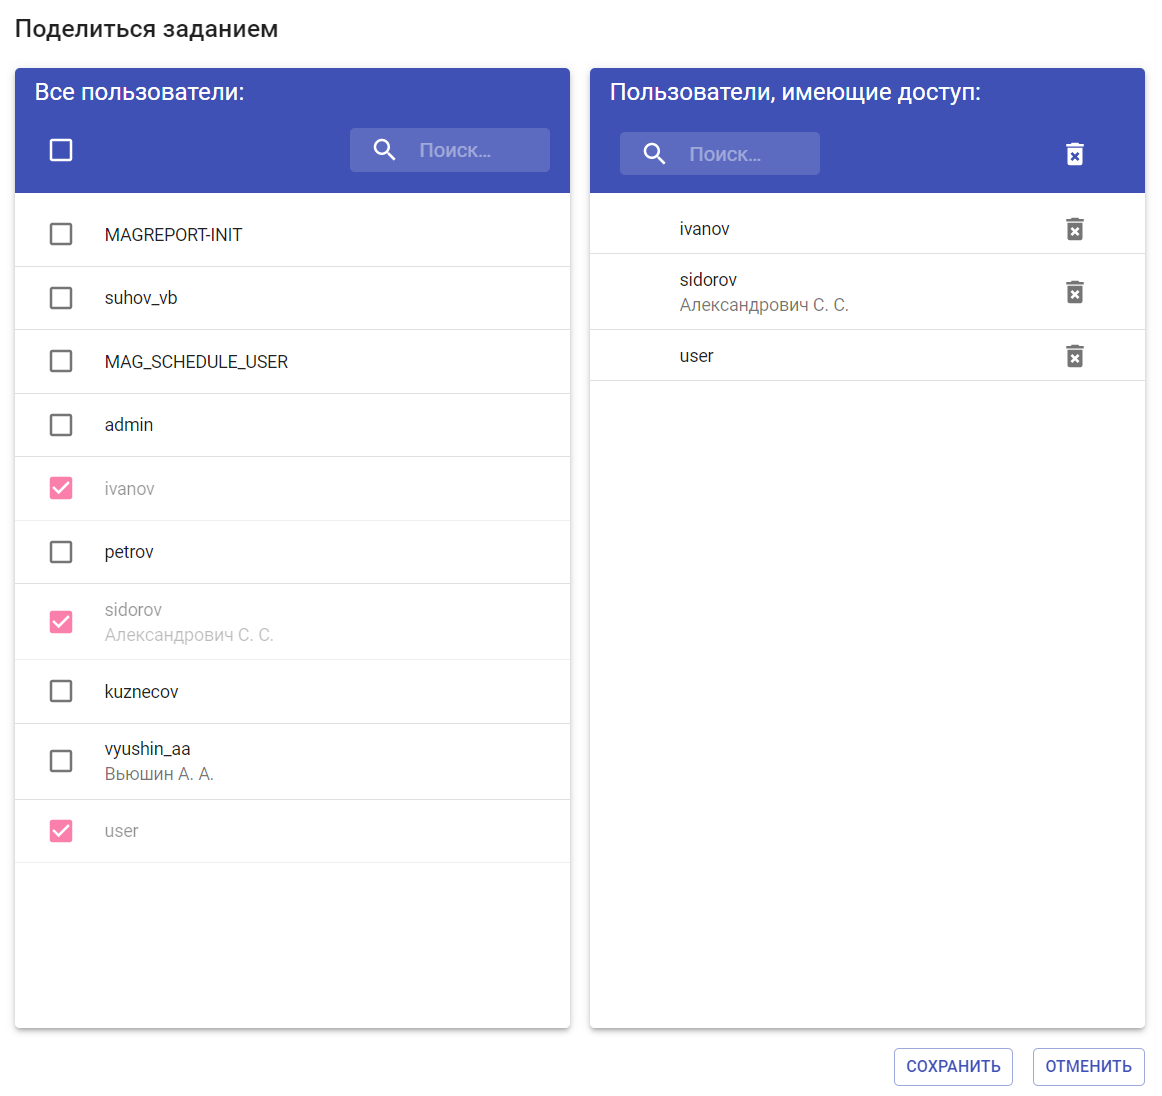
\includegraphics[width=\graphicswidth]{img/28-share-pivot.png}
		\caption{Выбор пользователей для расшаривания задания}
		\label{fig:share-pivot}
	\end{figure}	

	У пользователя, с которым поделились заданием, такое задание появится в разделе <<Задания>> вкладке <<Поделились со мной>> (см. рис. \ref{fig:shared-task}).
	
	\begin{figure}[h]
		\centering
		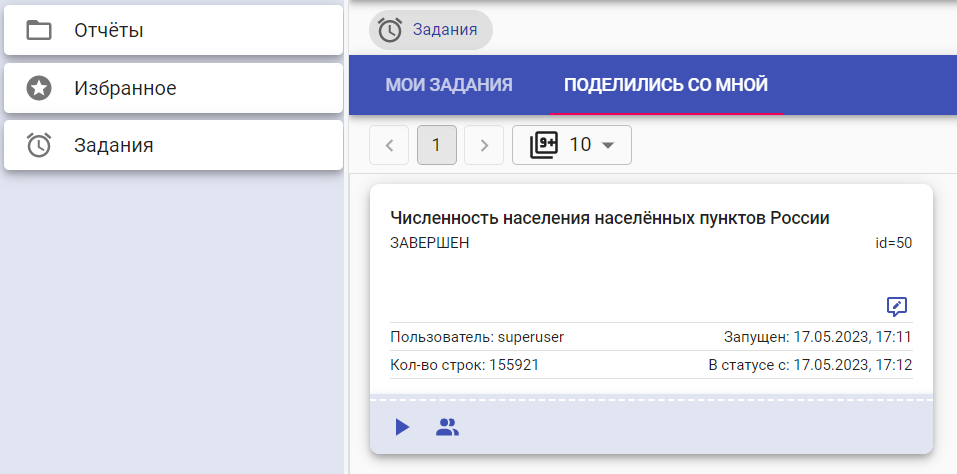
\includegraphics[width=\graphicswidth]{img/29-shared-task.png}
		\caption{Задания, которыми поделились с пользователем}
		\label{fig:shared-task}
	\end{figure}	
	
	\section{Описание кнопок меню работы со сводной таблицей}
	
	
	Основные кнопки при работе со сводной таблицей показаны на рисунке  \ref{fig:pivot-menu}

	\begin{figure}[h]
		\centering
		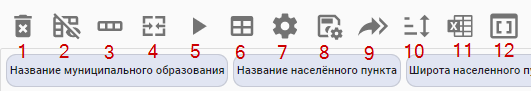
\includegraphics[width=\graphicswidth]{img/pivot-menu.png}
		\caption{Меню работы со сводной таблицей}
		\label{fig:pivot-menu}
	\end{figure}	
	
	\begin{enumerate}
		
		\item <<Очистить всё>> - очищает текущую конфигурацию сводной до начального (пустого) положения
		
		\item <<Скрыть панели с полями>> / <<Показать панели с полями>> - скрывает все панели с полями для увеличения области видимости сводной таблицы / отображает все панели с полями
		
		\item <<Метрики по столбцам>> / <<Метрики по строкам>> - переключение размещения метрик по столбцам или строкам
		
		\item <<Слить одинаковые>> / <<Разделить одинаковые>> - объединение одинаковых значений в строках и столбцах в единую ячейку / разделить одинаковые значения в ячейках для отображения в каждой строке
		
		\item <<Перезапустить отчёт>> - переход в раздел заполнения фильтров для выполнения отчета
		
		\item <<Простая таблица>> - переход в раздел с простой таблицей отчета
		
		\item <<Конфигурации>> - выбор конфигурации из существующих для данного отчета (задания)
		
		\item <<Сохранить конфигурацию>> - сохранение текущей конфигурации
		
		\item <<Поделиться заданием>> - переход в меню для возможности поделиться текущей конфигурацией с пользователем Магрепорт
		
		\item <<Сортировка>> - отображает настройки текущей сортировки, позволяет очистить текущую сортировку
		
		\item <<Экспорт в Excel>> - выгрузка текущей сводной в Excel в виде простой таблицы
		
		\item <<Производные поля>> - переход в раздел работы с производными полями
		
	\end{enumerate}
	
\end{document}